\documentclass[hyperref={xetex}]{beamer}
\title{Einführung in Matlab und Python - Einheit 8}
\subtitle{Schnittstelle zu C}
\mode<article>
{
  \usepackage{fullpage}
  \usepackage{pgf}
  \usepackage{hyperref}
  \setjobnamebeamerversion{beamer}
}

\mode<presentation>
{
  %\usetheme{Frankfurt}
 %\usetheme{My}
  \usetheme{Madrid}
  % or ...
%\usecolortheme{seagull}
  %\setbeamercovered{transparent}
  %\setbeamercovered{dynamic}
  % or whatever (possibly just delete it)
}
\usenavigationsymbolstemplate{}
\usefonttheme{structurebold}
\usepackage{multimedia}
\usepackage{tikz}
\usepackage{fontspec,xunicode,xltxtra}
%\usepackage[scaled=.90]{helvet}
% Or whatever. Note that the encoding and the font should match. If T1
% does not look nice, try deleting the line with the fontenc.

\setbeamertemplate{footline}
{
\leavevmode
%\hbox{\begin{beamercolorbox}[wd=.5\paperwidth,ht=2.5ex,dp=1.125ex,
%leftskip=.3cm plus1fill,rightskip=.3cm]{author in head/foot}%
%    \usebeamerfont{author in head/foot}\insertshortauthor
%  \end{beamercolorbox}%
%  \begin{beamercolorbox}[wd=.5\paperwidth,ht=2.5ex,dp=1.125ex,leftskip=.3cm,
%rightskip=.3cm plus1fil]{title in head/foot}%
%    \usebeamerfont{title in head/foot}\insertshorttitle\hfill

\hfill\insertframenumber  \hspace{3pt}

%\inserttotalframenumber
%\hspace*{2ex}
%  \end{beamercolorbox}}%
  \vskip3pt%
}

%\usepackage[english]{babel}
\usepackage[ngerman]{babel}
\selectlanguage{ngerman}

%
% math/symbols
%
\usepackage{amssymb}
\usepackage{amsthm}
% \usepackage{latexsym}
\usepackage{amsmath}
%\usepackage{listings}
\usepackage[framed]{mcode}
%\usepackage{mcode}

\usepackage{mydef}
\usepackage{cmap} % you can search in the pdf for umlauts and ligatures
%\usepackage{colonequals} %corrects the definition-symbols \colonequals (besides others)
\title{Einführung in Matlab}
%
%\subtitle{Disputation} % (optional)

\author{Jochen Schulz}
% - Use the \inst{?} command only if the authors have different
%   affiliation.

\institute{Georg-August Universit\"at G\"ottingen \pgfimage[height=0.5cm]{../figures/unilogo3}}
% - Use the \inst command only if there are several affiliations.
% - Keep it simple, no one is interested in your street address.

\date{\today}

\subject{Einführung in Matlab}
% This is only inserted into the PDF information catalog. Can be left
% out. 



% If you have a file called "university-logo-filename.xxx", where xxx
% is a graphic format that can be processed by latex or pdflatex,
% resp., then you can add a logo as follows:

%\logo{\pgfimage[height=0.5cm]{figures/unilogo3}}


% Delete this, if you do not want the table of contents to pop up at
% the beginning of each subsection:
% \AtBeginSubsection[]
% {
%   \begin{frame}<beamer>
%     \frametitle{Aufbau}
%     \tableofcontents[currentsection,currentsubsection]
%   \end{frame}
% }

\AtBeginSection[]
{
  \begin{frame}<beamer>
    \frametitle{Aufbau}
    \tableofcontents[currentsection,currentsubsection]
  \end{frame}
}


\begin{document}



\begin{document}
\titlepage

\section{Schnittstelle zu C}
%
% Slide
%
\begin{frame}[fragile]\frametitle{Schnittstellen in MATLAB}
\begin{itemize}
\item MATLAB l\"a{\ss}t sich mit anderen Programmiersprachen kombinieren. 
\item Die Verkn\"upfung geschieht \"uber sogenannte \alert{Schnittstellen} (engl. interfaces). 
\item Es existieren Schnittstellen zu C, Fortran und Java.
\item \"Uber diese Schnittstellen können Kommandos und Daten \"ubermittelt werden.
\end{itemize}
\end{frame}
%
% Slide
%
\begin{frame}[fragile]\frametitle{Warum Schnittstellen zu C?}
\begin{itemize}
\item \alert{Wiederverwendung}: Gro{\ss}e bereits existierende C-Programme k\"onnen von MATLAB aus
  gestartet werden, ohne dass sie als $m$-Files neugeschrieben werden
  m\"ussen. 
\item \alert{Performance}: Bottleneck Berechnungen (in der Regel Schleifen), die in MATLAB nicht
  schnell genug laufen, k\"onnen aus Effizienzgr\"unden in z.B. C neu programmiert
  werden. 
\item \alert{Stärken vereinen}: Man kann aus C-Programmen heraus, den Befehlsumfang von MATLAB nutzen (z.B. einfaches Erstellen von Grafiken).
\end{itemize}
\end{frame}

%
% Slide
%
\begin{frame}[fragile]\frametitle{Schnittstellen zu C}
Es gibt 2 M\"oglichkeiten, MATLAB mit C zu verbinden. 
\begin{itemize}
\item \textbf{Das Einbinden von C-Funktionen in MATLAB}\\ Dies geschieht durch die sogenannten
      \alert{mex-Dateien}. Sie bestehen aus 2 Teilen 
\begin{itemize}
\item  Schnittstellen-Routine zwischen C und MATLAB (Gateway).
\item \textit{eigentliche} $C$-Funktion
\end{itemize}

\item \textbf{Das Einbinden von MATLAB-Funktionen in C}\\ Hier bindet
      man passende Bibliotheken ein: die sogenannte \alert{Engine}.
\end{itemize}
\end{frame}
%
% Slide
%
\subsection{C aus MATLAB}
%
% Slide
%
\begin{frame}[fragile]\frametitle{Erstellen von Mex-Funktionen}
\begin{itemize}
\item Um eine Mex-Datei \mcode{mex_beispiel.c} ausf\"uhrbar zu machen, kompiliere
man es durch 
\begin{matlabin}
mex mex_beispiel.c
\end{matlabin}
\item Die Befehlseingabe kann sowohl im Command Window von  MATLAB als auch in einem beliebigen
  terminal (unter Linux) erfolgen (Pfad beachten).
\item Die Funktion kann dann in MATLAB aufgerufen werden als sei sie ein normales
m-File.
\end{itemize}
\end{frame}
%
% Slide
%
\begin{frame}[fragile]\frametitle{Erstellen von Mex-Funktionen}
\begin{itemize}
\item Mex-Dateien verhalten sich genau wie m-Files oder built-in Funktionen.
\item Mex-Dateien sind plattform-abh\"angig.
\item Die Plattform ist an der Endung zu erkennen:
\begin{itemize}
 \item \mcode{mexaxp} (Alpha)
\item \mcode{mexglx} (Linux)
\item \mcode{mexsol} (Solaris)
\item \mcode{dll} (Windows)
\end{itemize}
\end{itemize}
\end{frame}
%
% Slide
%
\begin{frame}[fragile]\frametitle{Optionen von mex}
\begin{itemize}
\item Ausw\"ahlen des Default-Compilers durch
\begin{matlabin}
mex -setup
\end{matlabin}
\item Es ist auch m\"oglich, von Fall zu Fall verschiedene Compiler zu
  benutzen. Aufruf:
\begin{matlabin}
mex filename -f optionsfile
\end{matlabin}
Beispiele: \mcode{lccengmatops.bat} (MATLAB-Compiler, Windows),
\mcode{gccopts.sh} (gcc, Linux) 
\item Weitere Informationen zum Aufruf von \mcode{mex}:
\begin{matlabin}
mex -help
\end{matlabin}
\end{itemize}
\end{frame}
%

% Slide
%
\begin{frame}[fragile]\frametitle{Linken mehrere Files}
\begin{itemize}
\item Beim Erzeugen von mex-Routinen ist es m\"oglich verschiedene Objekt- und
Bibliothek-Files zu kombinieren. \\
\textbf{Beispiel:}
\begin{matlabin}
mex circle.c square.obj rectangle.c 
    shapes.lib
\end{matlabin}
erzeugt unter Windows die ausf\"uhrbare Datei \mcode{circle.dll}. \\

\item Benutzen von Befehlen wie \mcode{make}
ist m\"oglich. 

\item Dateien werden am Ende durch \mcode{mex} zusammengebunden. 
\end{itemize}
\end{frame}
%
% Slide
%
\begin{frame}[fragile]\frametitle{Aufbau von mex-Files}
Sie bestehen aus 2 Teilen:
\begin{itemize}
 \item  Gateway Routine
\item eigentliche C-Funktion
\end{itemize}
Aufruf der Gateway-Funktion:
\begin{matlabin}[language=C++]
void mexFunction(
   int nlhs, mxArray *plhs[],
   int nrhs, const mxArray *prhs[])
\end{matlabin}

\end{frame}
%
% Slide
%
\begin{frame}[fragile]\frametitle{Gateway Routine}

\begin{itemize}
\item MATLAB Arrays f\"ur die Output Argumente zu erzeugen:
\begin{matlabin}[language=C++]
mxCreate
\end{matlabin}
\item Zeiger auf die neuerzeugten MATLAB-Arrays setzen:
\begin{matlabin}[language=C++]
plhs[0],[1],..
\end{matlabin}
\item Daten aus 
\begin{matlabin}[language=C++]
prhs[0],[1],.. 
\end{matlabin}
lesen:
\begin{matlabin}[language=C++]
mxGet
\end{matlabin}
\item Aufruf der $C$-Unterroutine mit den Input- und Output-Zeigern (\mcode{prhs},\mcode{plhs}) als
  Funktionsparameter. 
\end{itemize}
\end{frame}
%
% Slide
%
\begin{frame}[fragile]\frametitle{Arbeitsweise von mex-Files}
\begin{itemize}
\item Aufruf in MATLAB:
\begin{matlabin}
[C,D]=func_beispiel(A,B)
\end{matlabin}
Startet \mcode{func_beispiel.c}:
\begin{matlabin}[language=C++]
const mxArray *B,*A;
A = prhs[0];
B = prhs[1];

mxArray *C,*D;
C = plhs[0];
D = plhs[1];
\end{matlabin} 
\item Ergebnis MATLAB: \mcode{plhs[0]} wird in $C$ geschrieben, \mcode{plhs[1]}
  wird in $D$ geschrieben. 
\end{itemize}
\end{frame}

%
% Slide
% 
\begin{frame}[fragile]\frametitle{Klassifizierung von Funktionen}
\vspace*{-0.5cm}
Es gibt drei verschiedene Klassen von Funktionen im Zusammenhang mit der Schnittstelle.
\begin{itemize}
\item \alert{ mex-Funktionen:}\\
 Mex-Routinen interagieren mit der MATLAB Umgebung. 
Beispielsweise interpretiert \mcode{mexEvalString} einen String im MATLAB Workspace.  
\item \alert{ mx-Funktionen:} \\
Menge von Funktionen mit 
 denen man MATLAB Arrays erzeugen und manipulieren kann. 
\item \alert{ Engine Funktionen:}\\ 
 Menge von Funktionen, die das Arbeiten mit der MATLAB-Engine steuern. 
\end{itemize}
\end{frame}
%
%
%
\begin{frame}[fragile]\frametitle{Gr\"o{\ss}ter gemeinsamer Teiler (ggT)}
Berechnung des ggT von nat\"urlichen Zahlen $a$ und $b$ mit Hilfe des
euklidischen Algorithmus\\[1cm]

\alert{Idee:} Es gilt \alert{ $ggT(a,b)=ggT(a,b-a)$} f\"ur $a<b$.\\[1cm]

\alert{Algorithmus:} \\
Wiederhole,  bis $a=b$
\begin{itemize}
\item Ist $a>b$, so $a=a-b$.
\item Ist $a<b$, so $b=b-a$ 
\end{itemize}
\end{frame}

\begin{frame}[fragile]\frametitle{MATLAB}
\matinput{../einheit02/ggt.m}
\end{frame}
%
% Slide
% 
\begin{frame}[fragile]\frametitle{C-File: ggt.c (Teil I)}
\begin{matlabin}[language=C++]
/*******************************************
 *     ggt.c  
 *******************************************/
#include "mex.h"

void ggt( double   result[], double a, double b);

void mexFunction( int nlhs, mxArray *plhs[],
                  int nrhs, const mxArray *prhs[] )
{
  double *a,*b,*result;
  
  /* Erzeuge Matrix fuer das Rueckgabe-Argument. */
  plhs[0] = mxCreateDoubleMatrix(1,1, mxREAL);  
\end{matlabin}
\end{frame}
%
% Slide
% 
\begin{frame}[fragile]\frametitle{C-File: ggt.c (Teil II)}
\begin{matlabin}[language=C++]
  /* Die pointer fuer die Variablen  setzen */
  a = mxGetPr(prhs[0]);
  b = mxGetPr(prhs[1]);
  result = mxGetPr(plhs[0]);  
  /* Aufruf der ggt Routine */
  ggt ( result, *a, *b );
}

void ggt( double result[], double a, double b)
{
  while (a!=b)
  {
    if (a>b) 
      a = a - b;
    else
      b = b - a;      
  }
  result[0] = a;
}
\end{matlabin}
\end{frame}
%
% Slide
% 
\begin{frame}[fragile]\frametitle{Erkl\"arungen}
\begin{itemize}
\item Einbinden der Header Datei
\begin{matlabin}[language=C++]
#include "mex.h"
\end{matlabin}
\item Definieren eines Zeigers $x$ auf ein Objekt vom MATLAB-Typ \mcode{mxArray}. 
\begin{matlabin}[language=C++]
 mxArray *x = NULL;
\end{matlabin}
Zeiger vom Typ \mcode{mxArray} dienen zur abstrakten Zuweisung von MATLAB-Datenstrukturen.
\end{itemize}
\end{frame}
%
% Slide
% 
\begin{frame}[fragile]\frametitle{Erzeugen von  Rückgabe-strukturen}
\begin{itemize}
\item Definieren von \mcode{double}-Matrizen
\begin{matlabin}[language=C++]
mxArray *mxCreateDoubleMatrix(int m, int n, mxComplexity Flag);
\end{matlabin}
$m$ ist die Anzahl von Zeilen, $n$ die Anzahl von Spalten und \mcode{Flag} ist
entweder $mxREAL$ or $mxCOMPLEX$.
\item Definieren eines \mcode{double}-Skalars mit Wert \mcode{value}
\begin{matlabin}[language=C++]
mxArray *mxCreateDoubleScalar(double value);
\end{matlabin}
\end{itemize}
\end{frame}
%
% Slide
% 
\begin{frame}[fragile]\frametitle{Weitere Erzeuger}
\begin{center}
\begin{tabular}{|c|l|}
\hline
\mcode{mxCreateCellArray} & Array f\"ur Cell-Arrays \\
\mcode{mxCreateCharArray} & Array von Characters\\
\mcode{mxCreateString}    & String\\
\mcode{mxCreateSparse}    & Sparse Matrix \\ 
\mcode{mxCreateLogicalMatrix} & Array f\"ur Logicals\\
\hline
\end{tabular}
\end{center}
\end{frame}
%
% Slide
%
\begin{frame}[fragile]\frametitle{Zugriff auf mxArray}
\begin{matlabin}[language=C++]
double *mxGetPr(mxArray *array_zeiger)
\end{matlabin}
R\"uckgabeargument ist ein Zeiger, der auf das erste (reelle) Element des Arrays
\mcode{*array_ptr} zeigt. F\"ur imagin\"are Elemente \mcode{mxGetPi}. 
\end{frame}
%
% Slide
% 
\begin{frame}[fragile]\frametitle{Abfangen von Fehler}
Es findet keine automatische \"Uberpr\"ufung der Ein- und
  Ausgabeparameter statt. 2 M\"oglichkeiten:
\begin{itemize}
\item [(a)] Man versieht die Gateway-Routine mit entsprechenden Abfragen.
\item [(b)] Man kapselt die mex-Routine durch eine MATLAB-Routine, die die
  Parameter \"uberpr\"uft.
\end{itemize}
\end{frame}
%
% Slide
% 
\begin{frame}[fragile]\frametitle{C-File: ggt\_2.c (Auszug)}
\begin{matlabin}[language=C++]
/* Ueberpruefen der Anzahl von Argumenten */
  if(nrhs!=2) {
    mexErrMsgTxt("Genau 2 Input-Variablen erforderlich");
  } else if(nlhs!=1) {
    mexErrMsgTxt("Falsche Anzahl an Output-argumente");
  }
  /* Input Variablen muessen nichtnegative Double sein.*/
  mrows = mxGetM(prhs[0]);
  ncols = mxGetN(prhs[0]);
  if( !mxIsDouble(prhs[0]) || !(mrows==1 && ncols==1) ){
    mexErrMsgTxt("Erster Eingabeparameter muss 
      ein reelles Skalar sein.");
  }
  mrows = mxGetM(prhs[1]);
  ncols = mxGetN(prhs[1]);
  if( !mxIsDouble(prhs[1]) || !(mrows==1 && ncols==1) ){
    mexErrMsgTxt("Zweiter Eingabeparameter muss 
      ein reelles Skalar sein.");
  } 
\end{matlabin}
\end{frame}
%
% Slide
%
\begin{frame}[fragile]\frametitle{Befehle}
\begin{itemize}
\item Abfragen der Zeilen- bzw. Spaltenanzahl eines \mcode{mxArrays}:
\begin{matlabin}[language=C++]
int mxGetM(const mxArray *array_zeiger)
int mxGetN(const mxArray *array_zeiger)
\end{matlabin}
\item Fehlermeldung:
\begin{matlabin}[language=C++]
mexErrMsgTxt('Fehler....')
\end{matlabin}
erzeugt eine entsprechende Fehlermeldung in MATLAB und beendet die Routine. 
\end{itemize}
\end{frame}
%
% Slide
%
\begin{frame}[fragile]\frametitle{Typ-Abfragen}
\begin{matlabin}[language=C++]
bool mxIsDouble( mxArray *array_zeiger);
\end{matlabin}
\begin{itemize}
 \item wahr(1): wenn \mcode{*array_zeiger} eine Matrix mit \mcode{double} oder
\mcode{float} repr\"asentiert.
\item falsch(0): sonst
\end{itemize}

\alert{Weitere Abfragen:}  \\
\mcode{mxIsComplex}, \mcode{mxIsChar},
\mcode{mxIsInf}, \mcode{mxInt64}, \mcode{mxInt32}, \mcode{mxIsNaN}.
\end{frame}
%-------------------------------------------------
%  Folie:
%-------------------------------------------------
\begin{frame}[fragile]\frametitle{Mandelbrot-Menge}
Die Mandelbrot-Menge ist die Menge von Punkten $c \in \mathbb{C}$
bei denen die Folge $(z_n)_n$, die durch
\[ z_0:=c, \qquad  z_{n+1} = z_n^2 +c, \quad n \in \mathbb{N}\]
definiert ist, beschr\"ankt ist.
\begin{itemize}
\item Gilt $|z_n| \geq 2$, so wird die Folge divergieren.
\item Wir benutzen dies als Abbruchkriterium.
\end{itemize}
\end{frame}
\begin{frame}[fragile]\frametitle{Reelle Darstellung}
Mit $z=z_1+iz_2$, $x=x_1+ix_2$ und $c=c_1+ic_2$ ergibt sich aus
\begin{eqnarray*}
z_1 + i z_2 & = & z  =  x^2 + c = (x_1+ix_2)^2 + (c_1+ic_2) \\
& = & [ x_1^2 -x_2^2 +c_1] + i[2 x_1 x_2 +c_2]
\end{eqnarray*}
die Formel
\[ z_1 = x_1^2 -x_2^2 +c_1, \qquad z_2 = 2 x_1 x_2 + c_2. \]
\end{frame}
%-------------------------------------------------
%  Folie:
%-------------------------------------------------
\begin{frame}[fragile]\frametitle{Programm - MATLAB}
\begin{matlabin}
MAX_IT = 150;
x1 = linspace(-2.1,0.6,601);
y1 = linspace(-1.1,1.1,401);
C = zeros(length(y1),length(x1));
for i = 1:length(x1)
  for j = 1:length(y1)
    % Berechnen der Folge
    m = 0; a = x1(i); b = y1(j);
    x = a; y = b;
    while (sqrt(x^2+y^2)<2 && m<MAX_IT)
      t = x; x = a+x^2-y^2;
      y = b+2*t*y; m = m+1;
    end;
    C(j,i) = m;
  end
end
C = (1/MAX_IT) * C;
contourf(x1,y1,C,20);
\end{matlabin}
\end{frame}
%-------------------------------------------------
%  Folie:
%-------------------------------------------------
\begin{frame}[fragile]\frametitle{Routine - C (Teil I)}
\begin{matlabin}[language=C++]
#include "mex.h"
#include <math.h>

void mandel_c( double result[], double x1[], double y1[], 
  int x1_laenge,int y1_laenge);

void mexFunction( int nlhs, mxArray *plhs[],
int nrhs, const mxArray *prhs[] )
{
  double *a,*b,*result;
  int acols, bcols;

  acols = mxGetN(prhs[0]);
  bcols = mxGetN(prhs[1]);
\end{matlabin}
\end{frame}
%-------------------------------------------------
%  Folie:
%-------------------------------------------------
\begin{frame}[fragile]\frametitle{Routine - C (Teil II)}
\begin{matlabin}[language=C++]  
  printf("\n Erzeuge (%d x %d)-Matrix \n\n",bcols,acols);
    
  /* Erzeuge Matrix fuer das Rueckgabe-Argument. */
  plhs[0] = mxCreateDoubleMatrix(bcols,acols, mxREAL);

  /* Die pointer fuer die Variablen  setzen. */
  a = mxGetPr(prhs[0]);
  b = mxGetPr(prhs[1]);
  result = mxGetPr(plhs[0]);

  /* Aufruf der Routine */
  mandel_c ( result, a, b, acols, bcols);
}
\end{matlabin}
\end{frame}
%-------------------------------------------------
%  Folie:
%-------------------------------------------------
\begin{frame}[fragile]\frametitle{Routine - C (Teil III)}
\begin{matlabin}[language=C++]
void mandel_c( double result[], double x1[], double y1[], 
   int x1_laenge, int y1_laenge)
{
  int MAX_IT = 150;
  int i,j;
  double m,a,b,x,y,t;
  for (i =0;  i< x1_laenge; i++)
  {
    for (j = 0; j< y1_laenge; j++)
    {
      /* Berechnen der Folge */        
      while (sqrt(x*x+y*y)<2 & m<MAX_IT)
      {
       ...
      }
      result[i*y1_laenge+j] = m;
    }
  }
}
\end{matlabin}
\end{frame}
%-------------------------------------------------
%  Folie:
%-------------------------------------------------
\begin{frame}[fragile]\frametitle{Aufruf aus MATLAB}
\matinput{mandelbrot2.m}
\end{frame}
%-------------------------------------------------
%  Folie:
%-------------------------------------------------
\begin{frame}[fragile]\frametitle{Die Mandelbrotmenge}
\begin{center}
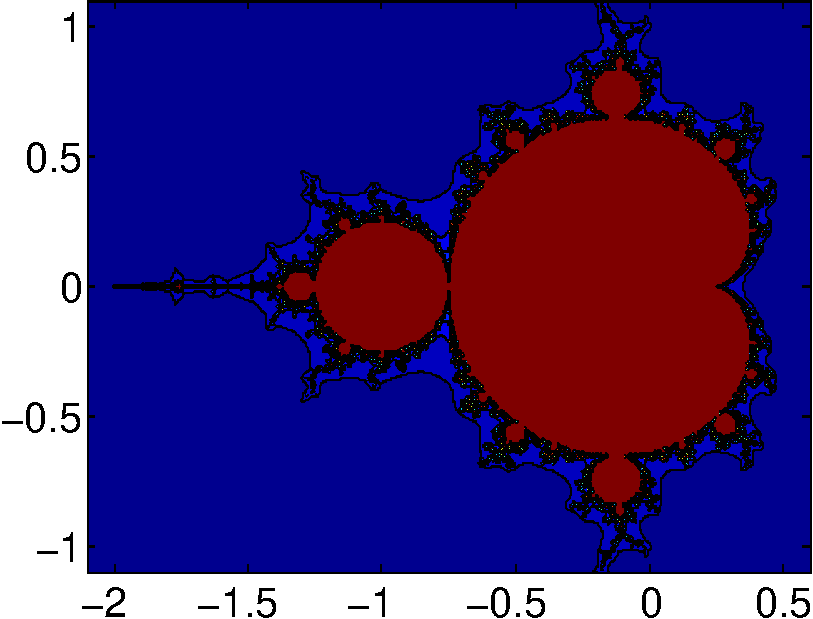
\includegraphics[width=0.8\textwidth]{./figures/mandelbrot}
\end{center}
\end{frame}
%
% Slide
%
\subsection{MATLAB aus C}
%
% Slide
%
\begin{frame}[fragile]\frametitle{Kompilieren unter Linux}

Befehle und Pfade gelten f\"ur MATLAB 2011b .

\begin{itemize}
%\item Einbinden der Shared Libraries (nur Linux, bash)
\item Bourne Shell
\begin{matlabin}[language=bash]
export LD_LIBRARY_PATH=/usr/local/matlab2011b/bin/glnx86/:/usr/local/matlab2011b/sys/os/glnx86:$LD_LIBRARY_PATH
\end{matlabin} %$
\begin{matlabin}[language=bash]
export LD_LIBRARY_PATH=/usr/local/matlab2011b/bin/glnxa64/:/usr/local/matlab2011b/sys/os/glnxa64:$LD_LIBRARY_PATH
\end{matlabin} %$


% \item C-Shell
% \begin{matlabin}[language=bash]
% setenv  LD_LIBRARY_PATH \
%   $MATLAB/bin/glnx86/:$LD_LIBRARY_PATH
% \end{matlabin}
\item Kompilieren von \mcode{test.c}
\begin{matlabin}[language=bash]
/usr/local/matlab2011b/bin/mex -f /usr/local/matlab2011b/bin/engopts.sh test.c
\end{matlabin}
oder
\begin{matlabin}[language=bash]
./compile test.c ; ./run test
\end{matlabin}

\end{itemize}
\end{frame}
% 
% Slide
% 
\begin{frame}[fragile]\frametitle{Kompilieren unter Windows}
\begin{itemize}
\item Aufruf in MATLAB von
\begin{matlabin}[language=bash]
mex -f lccengmatopts.bat datei.c
\end{matlabin}
kompiliert die Datei \mcode{datei.c}.
\item Starten durch Ausf\"uhren von \mcode{datei.exe}.
\item Alternativ ein DOS-Fenster \"offnen, ins richtige Verzeichnis wechseln  
 und dort das Programm durch Eingabe von \mcode{datei} starten.
\end{itemize}
\end{frame}
% 
% Slide
% 
%\begin{frame}[fragile]\frametitle{Anpassen des Systems}
%\begin{itemize}
%\item Kopieren Sie die Datei \mcode{/home/matlab01/.cshrc.linux} in das
%  Heimatverzeichnis
%\begin{matlabin}
%cp /home/matlab01/.cshrc.linux ~
%\end{matlabin}
%\item Öffnen Sie eine neue Shell.
%\item In der \alert{ neuen} Shell starten Sie MATLAB.  
%\end{itemize}
%\end{frame}
%
% Slide
%
\begin{frame}[fragile]\frametitle{Erstes Beispiel}
\begin{itemize}
\item Das C Programm \"offnet ein MATLAB Fenster.
\item Dort wird eine Hilbert-Matrix erzeugt.
\item Die Eigenwerte der Matrix werden berechnet.
\item Die Eigenwerte werden grafisch veranschaulicht.
\end{itemize}
\end{frame}
%
% Slide
%
\begin{frame}[fragile]\frametitle{hilbert1.c}
\begin{matlabin}[language=C++]
#include <stdio.h>
#include "engine.h"
 
main(int argc, char* argv[])
{
  Engine *ep;
  mxArray *x_m = NULL;
   
  double n=10;
      
  printf("\n Open MATLAB engine...\n");
  ep = engOpen(NULL);
     
  x_m = mxCreateDoubleMatrix(1, 1, mxREAL);
  *mxGetPr(x_m) = n;
\end{matlabin}
\end{frame}
%
%
%
\begin{frame}[fragile]\frametitle{hilbert1.c (Forts.)}
\begin{matlabin}[language=C++]   
  engPutVariable(ep,"x_m",x_m);
  engEvalString(ep,"a=hilb(x_m)");
  engEvalString(ep,"semilogy(eig(a),'*')");
     
  printf("Please press Return \n");
  fgetc(stdin);
  engClose(ep);
}
\end{matlabin}
\end{frame}
%
% Slide
%
\begin{frame}[fragile]\frametitle{Umgang mit der MATLAB-Engine}
\begin{itemize}
\item Einbinden der Bibliothek 
\begin{matlabin}[language=C++]
#include "engine.h"
\end{matlabin}
\item Anlegen eines Handles f\"ur die MATLAB-Engine
\begin{matlabin}[language=C++]
Engine *ep;
\end{matlabin}
\item \"Offnen der MATLAB-Engine
\begin{matlabin}[language=C++]
engOpen(NULL) 
\end{matlabin} 
\item Schliessen der MATLAB-Engine: 
\begin{matlabin}[language=C++]
engClose(ep);
\end{matlabin}
\end{itemize}
\end{frame}
%
% Slide
%
\begin{frame}[fragile]\frametitle{Arbeiten mit der MATLAB-Engine}
\begin{itemize}
\item  Benenne die Variable 'name' in MATLAB. Die Variable wird mit den Daten
\mcode{werte} versehen. 
\begin{matlabin}[language=C++]
 engPutVariable(ep,"name",werte);
\end{matlabin}
\item Ausf\"uhren von MATLAB-Befehlen:
\begin{matlabin}[language=C++]
engEvalString(ep,"Befehl");
\end{matlabin}
Startet das Kommando \mcode{Befehl} in der MATLAB-Engine \mcode{ep}.
\end{itemize}
\end{frame}
%
% Slide
%
\begin{frame}[fragile]\frametitle{Zweites Beispiel}
\begin{itemize}
\item Das C Programm \"offnet ein MATLAB Fenster.
\item Dort wird eine Hilbert-Matrix erzeugt.
\item Die Eigenwerte der Matrix werden berechnet.
\item Die Eigenwerte werden an das C-Programm zur\"uckgegeben und dort
  ausgegeben. 
\end{itemize}
\end{frame}
%
% Slide
%
\begin{frame}[fragile]\frametitle{hilbert2.c (Teil I)}
\begin{matlabin}[language=C++]
#include <stdio.h>
#include "engine.h"
 
main(int argc, char* argv[])
{
  Engine *ep;
  mxArray *x_m = NULL;
  mxArray *d = NULL, *le = NULL;
  double *Dreal;
  double laenge;
  int i;
     
  double n=10;
      
  printf("\n Open MATLAB engine...\n");
  ep = engOpen(NULL);
\end{matlabin}
\end{frame}
%
% Slide
%
\begin{frame}[fragile]\frametitle{hilbert2.c (Teil II)}
\begin{matlabin}[language=C++]
  x_m = mxCreateDoubleMatrix(1, 1, mxREAL);
  *mxGetPr(x_m) = n;
     
  engPutVariable(ep,"x_m",x_m);
  engEvalString(ep,"d=eig(hilb(x_m))");
  engEvalString(ep,"le=length(d)");
     
  d = engGetVariable(ep, "d");
  le = engGetVariable(ep,"le");
\end{matlabin}
\end{frame}
%
% Slide
%
\begin{frame}[fragile]\frametitle{hilbert2.c (Teil III)}
\begin{matlabin}[language=C++]     
  Dreal = mxGetPr(d);
  laenge = *mxGetPr(le);
    
  engClose(ep);
     
  for (i=0; i<laenge; i++)
  {
    printf ( "%d. Eigenwert %g \n" , i+1,Dreal[i] );
  }
     
  mxDestroyArray(x_m);
  mxDestroyArray(d);
}    
\end{matlabin}
\end{frame}
%
% Slide
% 
\begin{frame}[fragile]\frametitle{Erkl\"arungen}
\begin{itemize}
\item Kopieren der Variable $d$ aus dem MATLAB-Workspace in das C-Programm.
\begin{matlabin}[language=C++]
mxArray *engGetVariable(ep, "d");
\end{matlabin}
\item Freigeben des Speichers (Wichtig!)
\begin{matlabin}[language=C++]
mxDestroyArray(mxArray *x_m);
\end{matlabin}
\end{itemize}
\end{frame}
%
% Slide
%
\begin{frame}[fragile]\frametitle{Beispielprogramm}
\begin{itemize}
\item \mcode{plot_poisson.c} plottet die Funktion\\
$f(x,y)= \sin(4 \pi x) \sin (2 \pi y)$
auf $[0,1] \times [0,1]$.
\item In C betrachten wir das Gitter, das durch Zerlegen der x- und der
y-Richtung in 50 Punkten entsteht. 
\item Dann berechnen wir die Funktionswerte in C.
\item Das Gitter und die berechneten Vektoren werden an MATLAB \"ubergeben.
\item Dort wird die L\"osung mit Hilfe des Befehls \mcode{surf} gezeichnet.
\end{itemize}
\end{frame}
%
% Slide
%
\begin{frame}[fragile]\frametitle{plot-poisson.c (Teil I)}
\begin{matlabin}[language=C++]
/*-----------------------------------------
 * -       plot_poisson.c
 * -----------------------------------------------*/

#include <stdio.h>
#include <math.h>
#include <string.h>
#include "engine.h"

#define MAX_ORDER 50

/* Function for plotting data on cartesian grids */
int plot_graph(
  double *x,   /* vector of x-values             */
  double *y,   /* vector of y-values             */
  double *z,   /* value at (x[i],y[j]) (row-wise)*/
  int    x_n,  /* size of array x                */
  int    y_n); /* size of array y                */
\end{matlabin}
\end{frame}
%
% Slide
%
\begin{frame}[fragile]\frametitle{plot-poisson.c (Teil II)}
\begin{matlabin}[language=C++]
/*---------------------------------------------------
-             main program                          -     
-----------------------------------------------------*/
main(int argc, char* argv[]) 
{
  double x[MAX_ORDER];
  double y[MAX_ORDER];
  double z[MAX_ORDER*MAX_ORDER];
  int x_n,y_n;
  int i,j;        
  x_n = 50;
  y_n = 50;
\end{matlabin}
\end{frame}
%
% Slide
%
\begin{frame}[fragile]\frametitle{plot-poisson.c (Teil III)}
\begin{matlabin}[language=C++]  
for (i=0; i<x_n; i++)
{
  x[i] = (double) i/(x_n-1);
}
for (i = 0; i<y_n; i++)
{
  y[i] = (double) i/(y_n-1);
}
for (i = 0; i<x_n; i++) 
{
  for (j = 0; j<y_n; j++)
  {
    *(z+i+j*x_n) = sin(4*3.14159*x[i])*sin(2*3.141459*y[j]);
  }
}      
if (plot_graph(x,y,z,x_n,y_n)==0) 
  printf("\n Ungueltiger Aufruf von 'plot_graph' \n");
return  0; }
\end{matlabin}
\end{frame}
%
% Slide
%
\begin{frame}[fragile]\frametitle{plot-poisson.c (Teil IV)}
\begin{matlabin}[language=C++]     
/*-------- function 'plot_graph' -----------*/
int plot_graph(double *x, double *y, double *z, int x_n, int y_n)
{  
  Engine *ep;
  mxArray *x_m = NULL;
  mxArray *y_m = NULL;
  mxArray *z_m = NULL;
  int i,j;
  if ((x_n ==0) || (y_n==0))  return (int) 0;
  printf("\n Open MATLAB engine...\n");
  if (!(ep = engOpen("\0"))) {
    fprintf(stderr, "\n Can't start MATLAB engine\n");
    return EXIT_FAILURE;
  }
  printf("Create MATLAB arrays...\n");
  x_m = mxCreateDoubleMatrix(1, x_n, mxREAL);
  y_m = mxCreateDoubleMatrix(1, y_n, mxREAL);
  z_m = mxCreateDoubleMatrix(x_n, y_n, mxREAL);
\end{matlabin}
\end{frame}
%
% Slide
%
\begin{frame}[fragile]\frametitle{plot-poisson.c (Teil V)}
\begin{matlabin}[language=C++]     
  printf("Copy entries into MATLAB ...\n");
  memcpy((void *)mxGetPr(x_m), (void *) x, x_n*sizeof(double));
  memcpy((void *)mxGetPr(y_m), (void *) y, y_n*sizeof(double));
  memcpy((void *)mxGetPr(z_m), (void *) z, x_n*y_n*sizeof(double));      
  engPutVariable(ep,"x_m",x_m);
  engPutVariable(ep,"y_m",y_m);
  engPutVariable(ep,"z_m",z_m);     
  printf("Execute MATLAB commands...\n");
  engEvalString(ep,"[Y,X]=meshgrid(y_m,x_m)");
  engEvalString(ep,"surf(X,Y,z_m)");
  engEvalString(ep,"xlabel('x')");
  engEvalString(ep,"ylabel('y')"); 
  printf("Please press Return \n");
  fgetc(stdin);  
  printf("\n Close MATLAB engine... \n");
  engClose(ep);  return (int) 1; }  
\end{matlabin}
\end{frame}
\end{document}

